\chapter{Testing and data analysis}\label{sec:TestingAndDataAnalysis}
This chapter goal is to show application testing, data collection and analysis.

\section{Testing environment}\label{sec:TestingEnvironment}
Test site of this application is a third floor of the Campus building of the Faculty of Informatics and Management, University of Hradec Kralove (FIM UHK). The main walk-through corridors are in a rectangular arrangement. Classrooms and offices are situated inwards and outwards in relation to the corridors. There is a roofed atrium in the center of the building. Experiments have been conducted in a 52 m x 43 m area.

\begin{figure}[H]
	\begin{centering}
		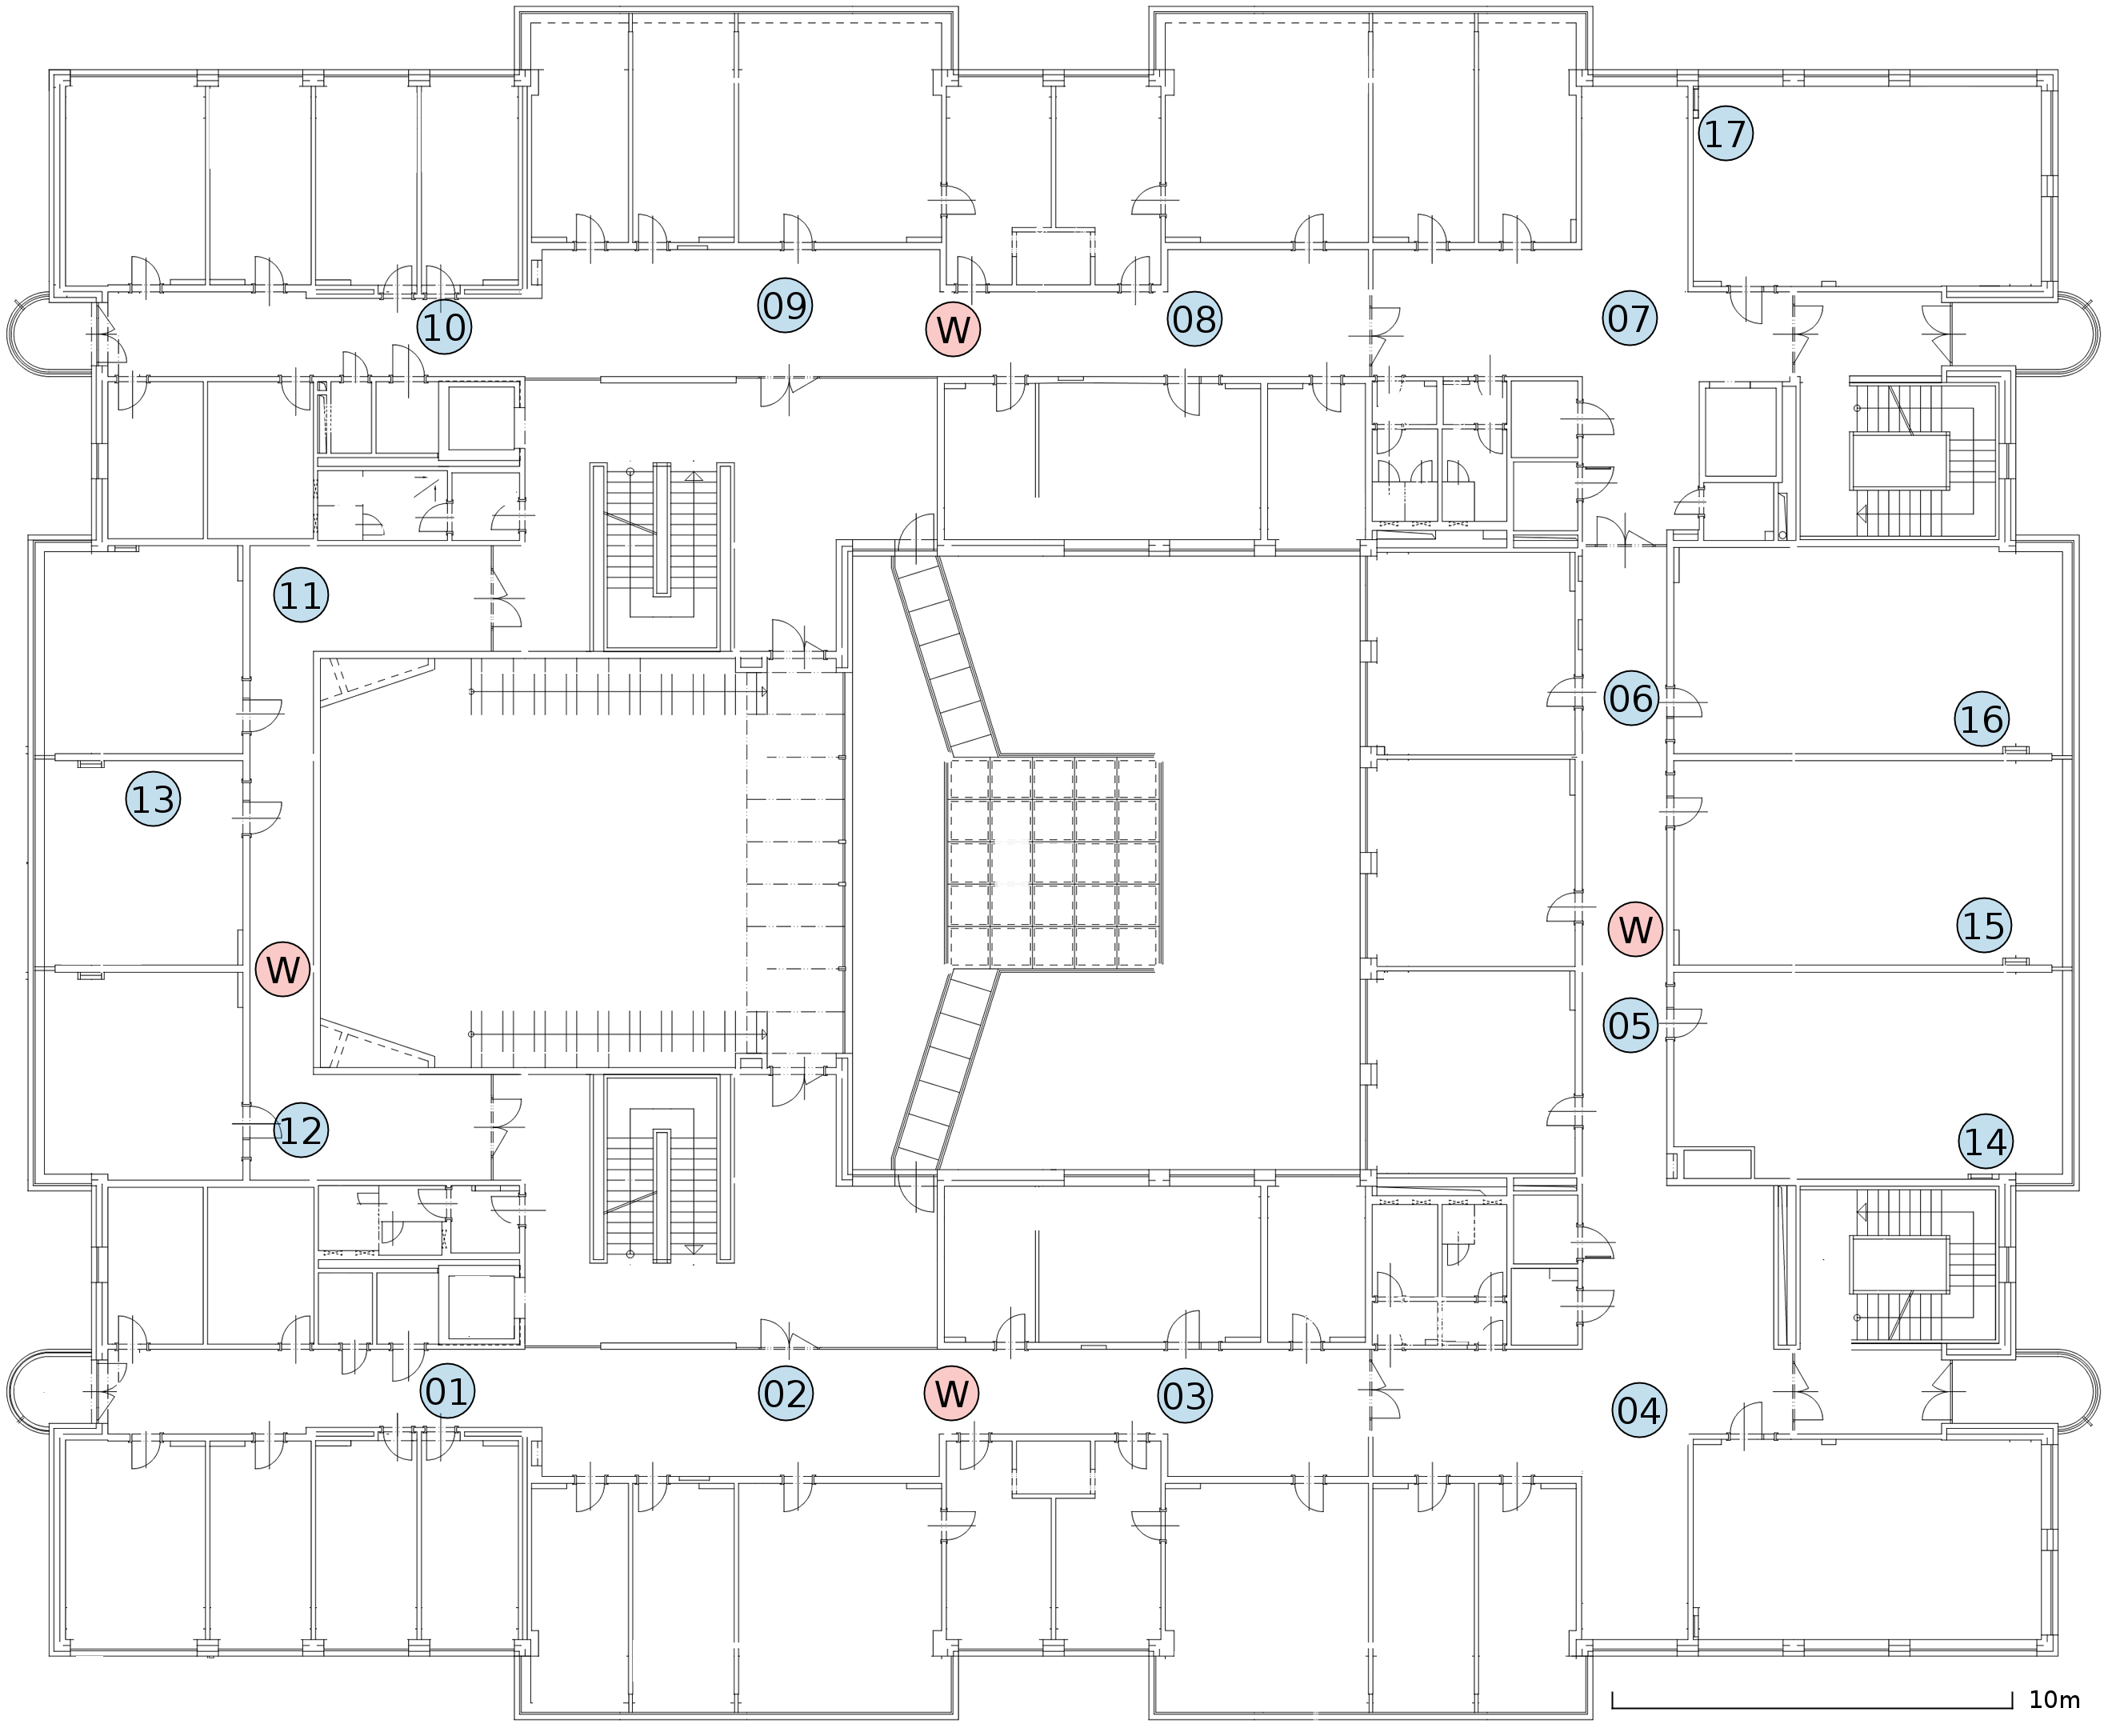
\includegraphics[width=0.8\textwidth]{img/j3np}
		\par\end{centering}
	\caption{Map of deployed devices (based on \cite{IILUBLEB})}
	\label{fig01c06}
\end{figure}

\fref{fig01c06} shows positions of deployed devices. There are four WiFi transmitters for \verb|eduroam| network made by Cisco (marked as W) on this floor. They are permanently placed on the ceiling and their settings could not be altered. Each marked place has usually more than one of them, typically at least two. One of them broadcasting in a 2.4 GHz and the other in a 5 GHz band. Their TX and power is automatically adjusted to help mitigate interference and signal coverage problems.

The other devices marked by numbers from 1 to 17 are Bluetooth Low Energy beacons placed evenly in the corridors and on the floor. They broadcast parameters were set to the advertising interval of 100 ms and the TX power of 0 dBm. Corridor beacons are placed in positions about 10 m apart from others \cite{IILUBLEB}. Since the beacons were placed two years ago there was a possibility of battery depletion and malfunction. By multiple tests we figured that two beacons had their battery depleted (1, 4), one was reconfigured and one was missing completely (5).

\section{Data collection}\label{sec:DataCollection}
Data was collected at 105 evenly-spaced (2m) positions of Campus building floor. Each position was measured four times, in two different headings (north, south) and with two device orientations, to prevent signal obstruction. Using two devices, 105 positions and 4 scans per position resulted in 840 different measurements consisting of 540,168 individual RSSI samples.

Each of the scans was run for 30 seconds on both devices at the same time to provide equal environment. It is not really feasible to run such long scans in one run so the decision was made to split sub-scans into smaller time intervals. BLE beacons have advertising interval set to 100 ms and single scan length could be set to same but it is set to 200 ms to prevent packet loss between the scans. Since localization using WiFi usually does not need big amount of data, scanner is set to run every 5 minutes. Same time is set for cellular and sensor scanner since this data is used only as complimentary and it helps to reduce fingerprint data size.

\section{Analysis}\label{sec:Analysis}